% !TEX TS-program = knitr
\documentclass{beamer}\usepackage{graphicx, color}
%% maxwidth is the original width if it is less than linewidth
%% otherwise use linewidth (to make sure the graphics do not exceed the margin)
\makeatletter
\def\maxwidth{ %
  \ifdim\Gin@nat@width>\linewidth
    \linewidth
  \else
    \Gin@nat@width
  \fi
}
\makeatother

\IfFileExists{upquote.sty}{\usepackage{upquote}}{}
\definecolor{fgcolor}{rgb}{0.2, 0.2, 0.2}
\newcommand{\hlnumber}[1]{\textcolor[rgb]{0,0,0}{#1}}%
\newcommand{\hlfunctioncall}[1]{\textcolor[rgb]{0.501960784313725,0,0.329411764705882}{\textbf{#1}}}%
\newcommand{\hlstring}[1]{\textcolor[rgb]{0.6,0.6,1}{#1}}%
\newcommand{\hlkeyword}[1]{\textcolor[rgb]{0,0,0}{\textbf{#1}}}%
\newcommand{\hlargument}[1]{\textcolor[rgb]{0.690196078431373,0.250980392156863,0.0196078431372549}{#1}}%
\newcommand{\hlcomment}[1]{\textcolor[rgb]{0.180392156862745,0.6,0.341176470588235}{#1}}%
\newcommand{\hlroxygencomment}[1]{\textcolor[rgb]{0.43921568627451,0.47843137254902,0.701960784313725}{#1}}%
\newcommand{\hlformalargs}[1]{\textcolor[rgb]{0.690196078431373,0.250980392156863,0.0196078431372549}{#1}}%
\newcommand{\hleqformalargs}[1]{\textcolor[rgb]{0.690196078431373,0.250980392156863,0.0196078431372549}{#1}}%
\newcommand{\hlassignement}[1]{\textcolor[rgb]{0,0,0}{\textbf{#1}}}%
\newcommand{\hlpackage}[1]{\textcolor[rgb]{0.588235294117647,0.709803921568627,0.145098039215686}{#1}}%
\newcommand{\hlslot}[1]{\textit{#1}}%
\newcommand{\hlsymbol}[1]{\textcolor[rgb]{0,0,0}{#1}}%
\newcommand{\hlprompt}[1]{\textcolor[rgb]{0.2,0.2,0.2}{#1}}%

\usepackage{framed}
\makeatletter
\newenvironment{kframe}{%
 \def\at@end@of@kframe{}%
 \ifinner\ifhmode%
  \def\at@end@of@kframe{\end{minipage}}%
  \begin{minipage}{\columnwidth}%
 \fi\fi%
 \def\FrameCommand##1{\hskip\@totalleftmargin \hskip-\fboxsep
 \colorbox{shadecolor}{##1}\hskip-\fboxsep
     % There is no \\@totalrightmargin, so:
     \hskip-\linewidth \hskip-\@totalleftmargin \hskip\columnwidth}%
 \MakeFramed {\advance\hsize-\width
   \@totalleftmargin\z@ \linewidth\hsize
   \@setminipage}}%
 {\par\unskip\endMakeFramed%
 \at@end@of@kframe}
\makeatother

\definecolor{shadecolor}{rgb}{.97, .97, .97}
\definecolor{messagecolor}{rgb}{0, 0, 0}
\definecolor{warningcolor}{rgb}{1, 0, 1}
\definecolor{errorcolor}{rgb}{1, 0, 0}
\newenvironment{knitrout}{}{} % an empty environment to be redefined in TeX

\usepackage{alltt}
\newcommand{\answers}{1}

\usetheme{Marburg}
\setbeamertemplate{navigation symbols}{} 
\setbeamercovered{dynamic}
\setbeamertemplate{footline}
{
  \leavevmode%
  \hbox{%
  \begin{beamercolorbox}[wd=.333333\paperwidth,ht=2.25ex,dp=1ex,center]{author in head/foot}%
    \usebeamerfont{author in head/foot}\copyright $\ $ \insertshortauthor%~~\beamer@ifempty{\insertshortinstitute}{}{(\insertshortinstitute)}
  \end{beamercolorbox}%
  \begin{beamercolorbox}[wd=.333333\paperwidth,ht=2.25ex,dp=1ex,center]{title in head/foot}%
    \usebeamerfont{title in head/foot} \insertinstitute
  \end{beamercolorbox}%
  \begin{beamercolorbox}[wd=.333333\paperwidth,ht=2.25ex,dp=1ex,right]{date in head/foot}%
    \usebeamerfont{date in head/foot}\insertshortdate{}\hspace*{2em}
    \insertframenumber{} / \inserttotalframenumber\hspace*{2ex} 
  \end{beamercolorbox}}%
  \vskip0pt%
}

\usepackage{amsmath}
\usepackage{caption}
\usepackage{color}
\usepackage{enumerate}
\usepackage{listings}
\usepackage{hyperref}
\usepackage{mathrsfs}
\usepackage{natbib}
\usepackage{url}

\providecommand{\all}{\ \forall \ }
\providecommand{\bs}{\backslash}
\providecommand{\e}{\varepsilon}
\providecommand{\E}{\ \exists \ }
\providecommand{\lm}[2]{\lim_{#1 \rightarrow #2}}
\providecommand{\m}[1]{\mathbb{#1}}
\providecommand{\nv}{{}^{-1}}
\providecommand{\ov}[1]{\overline{#1}}
\providecommand{\p}{\newpage}
\providecommand{\q}{$\quad$ \newline}
\providecommand{\rt}{\rightarrow}
\providecommand{\Rt}{\Rightarrow}
\providecommand{\vc}[1]{\boldsymbol{#1}}
\providecommand{\wh}[1]{\widehat{#1}}

\hypersetup{colorlinks,linkcolor=,urlcolor=blue}
\numberwithin{equation}{section}

\definecolor{dkgreen}{rgb}{0,0.6,0}
\definecolor{gray}{rgb}{0.5,0.5,0.5}
\definecolor{mauve}{rgb}{0.58,0,0.82}

\lstset{ 
  language=C,                % the language of the code
  basicstyle= \footnotesize,           % the size of the fonts that are used for the code
  numberstyle= \tiny \color{white},  % the style that is used for the line-numbers
  stepnumber=2,                   % the step between two line-numbers. 
  numbersep=5pt,                  % how far the line-numbers are from the code
  backgroundcolor=\color{white},      % choose the background color. You must add \usepackage{color}
  showspaces=false,               % show spaces adding particular underscores
  showstringspaces=false,         % underline spaces within strings
  showtabs=false,                 % show tabs within strings adding particular underscores
  frame=lrb,                   % adds a frame around the code
  rulecolor=\color{black},        % if not set, the frame-color may be changed on line-breaks within not-black text 
  tabsize=2,                      % sets default tabsize to 2 spaces
  captionpos=t,                   % sets the caption-position 
  breaklines=true,                % sets automatic line breaking
  breakatwhitespace=false,        % sets if automatic breaks should only happen at whitespace
  %title=\lstname,                   % show the filename of files included with \lstinputlisting;
  keywordstyle=\color{blue},          % keyword style
  commentstyle=\color{gray},       % comment style
  stringstyle=\color{dkgreen},         % string literal style
  escapeinside={\%*}{*)},            % if you want to add LaTeX within your code
  morekeywords={*, ...},               % if you want to add more keywords to the set
  xleftmargin=0.053in, % left horizontal offset of caption box
  xrightmargin=-.03in % right horizontal offset of caption box
}

%\DeclareCaptionFont{white}{\color{white}}
%\DeclareCaptionFormat{listing}{\parbox{\textwidth}{\colorbox{gray}{\parbox{\textwidth}{#1#2#3}}\vskip-0.05in}}
%\captionsetup[lstlisting]{format = listing, labelfont = white, textfont = white}
%For caption-free listings, comment out the 3 lines above and uncomment the 2 lines below.
 \captionsetup{labelformat = empty, labelsep = none}
 \lstset{frame = single}





\title{Descriptive Statistics: Part 2/2 (Ch 3)}
\author{Will Landau}
\date{January 24, 2013}
\institute{Iowa State University}

\begin{document}

\begin{frame}
\titlepage
 \end{frame}
 
 \AtBeginSection[]
{
   \begin{frame}
       \frametitle{Outline}
       \tableofcontents[currentsection]
   \end{frame}
}


\section{Boxplots}

\begin{frame}
\frametitle{Generic Boxplot}
\begin{center}
\setkeys{Gin}{width=1.048\textwidth} 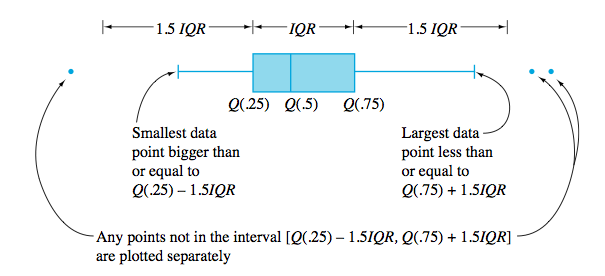
\includegraphics{../../fig/genericbox.png}
\end{center}
\end{frame}

\begin{frame}
\frametitle{Example: bullet data}
\begin{center}
\setkeys{Gin}{width= .75\textwidth} 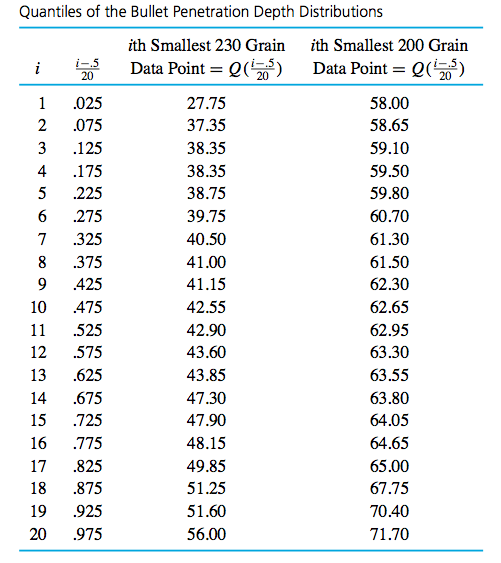
\includegraphics{../../fig/bulletquantiles.png}
\end{center}
\end{frame}

\begin{frame}
\frametitle{Example: bullet data (230-grain bullets)}
\begin{center}
\setkeys{Gin}{width= 1\textwidth} 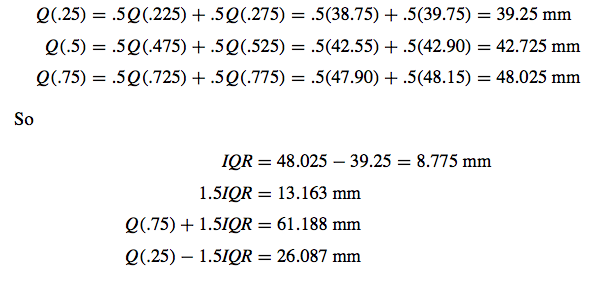
\includegraphics{../../fig/bulletquartiles.png}
\end{center}
\end{frame}

\begin{frame}
\frametitle{Example: bullet data}
\begin{center}
\setkeys{Gin}{width= .75\textwidth} 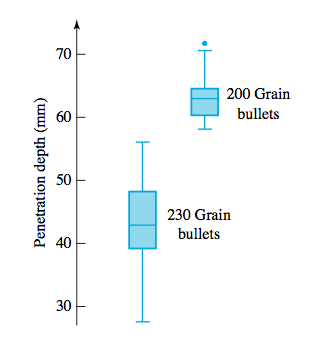
\includegraphics{../../fig/bulletbox.png}
\end{center}
\end{frame}


\section{Quantile-Quantile (QQ) Plots}

\begin{frame}
\frametitle{}
\begin{itemize}
\item {\bf Quantile-quantile (QQ) plot}: a scatterplot of the sorted values of one dataset on the sorted values of another dataset.
\begin{itemize}
\pause \item This plot is used to tell if the distributional shapes of the datasets are the same or different.
\begin{itemize}
\pause \item  If the points in the plot lie in a straight line, the distributional shapes are the same.
\pause \item Otherwise, the shapes are different.
\end{itemize}
\pause \item The datasets must be univariate, numerical, and of the same size.
\end{itemize}
\end{itemize}
\end{frame}

\begin{frame}
\frametitle{Example: bullet data}
\begin{center}
\setkeys{Gin}{width= .75\textwidth} 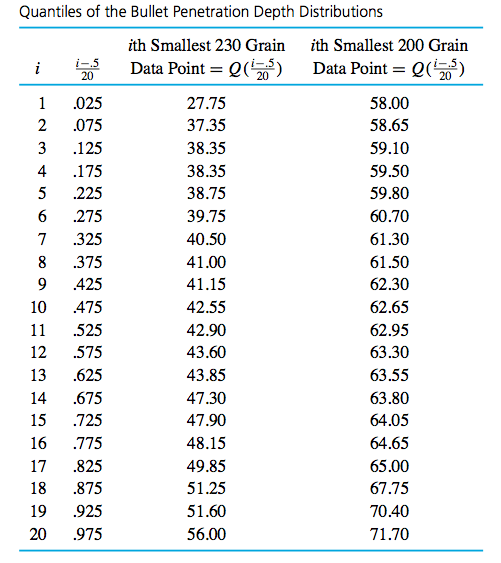
\includegraphics{../../fig/bulletquantiles.png}
\end{center}
\end{frame}

\begin{frame}
\frametitle{Example: bullet data} \small
\begin{itemize}
\item I can make a QQ plot of the bullet data by plotting the sorted 200-grain depths against the sorted 230-grain depths.
\pause \item The points lie in approximately a straight line, so the 200-grain depths are similarly shaped in distribution to the 230-grain depths.
\end{itemize}

\begin{center}
\setkeys{Gin}{width= .75\textwidth} 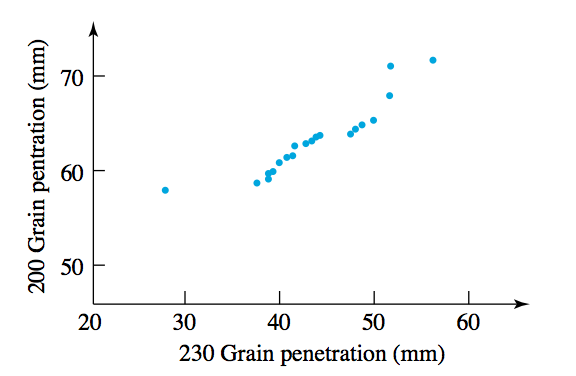
\includegraphics{../../fig/bulletqq.png}
\end{center}
\end{frame}


\section{Theoretical Quantile-Quantile Plots}

\begin{frame}
\frametitle{Theoretical quantile-quantile (QQ) plots}

\begin{itemize}
\item {\bf Theoretical quantile-quantile (QQ) plot}: a scatterplot with:
\begin{itemize}
\pause \item The sorted values $x_1, x_2, \ldots x_n$ of some real data set on the $x$ axis.
\pause \item $Q(\frac{1 - .5}{n}), Q(\frac{2 - .5}{n}), \ldots, Q(\frac{n - .5}{n})$ on the $y$ axis.
\begin{itemize}
\pause \item $Q$ is some {\bf theoretical quantile function}: the quantile function we would \emph{expect} from a dataset if that dataset had a certain shape.
\end{itemize}
\end{itemize}

\pause \item Example theoretical quantile functions:
\begin{itemize}
\pause \item ``Standard" bell-shaped data should have:
\begin{align*}
Q(p) \approx 4.9(p^{0.14} - (1 - p)^{0.14})
\end{align*}
\pause \item ``Exponentially distributed" data (a kind of highly right-skewed data) should have:
\begin{align*}
Q(p) \approx - \lambda \nv \log(1-p)
\end{align*}
where $\lambda$ is some constant.
\end{itemize}
\end{itemize}
\end{frame}

\begin{frame}
\frametitle{Normal quantile-quantile (QQ) Plots}
\begin{itemize}
\item {\bf Normal quantile-quantile (QQ) plot}: a theoretical QQ plot where the quantile function, $Q$, is the quantile function for ``standard" bell-shaped (normally-distributed) data.
\pause \item If the points in a normal QQ plot are in a straight line, the dataset in question is bell-shaped. Otherwise, the data is not bell-shaped.
\end{itemize}
\end{frame}

\begin{frame}
\frametitle{Example: towel breaking strength data}
\begin{center}
\setkeys{Gin}{width= .75\textwidth} 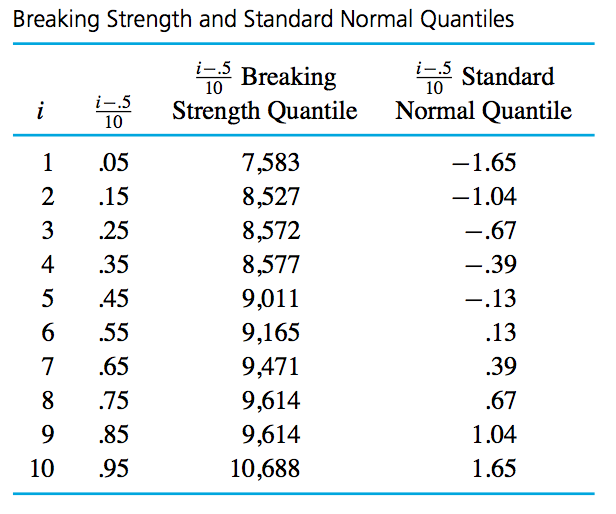
\includegraphics{../../fig/towelqqdata.png}
\end{center}
\end{frame}

\begin{frame}
\frametitle{Example: towel breaking strength data}
\begin{center}
\setkeys{Gin}{width= .7\textwidth} 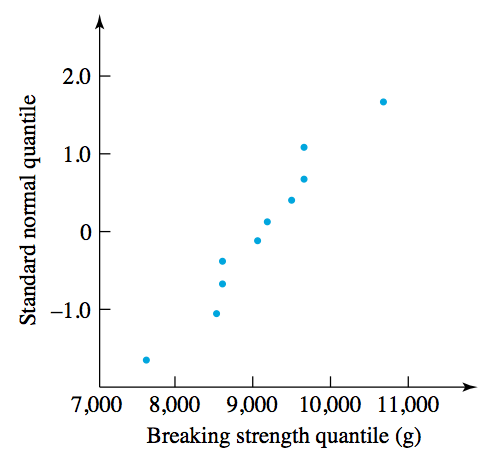
\includegraphics{../../fig/towelqqplot.png}
\end{center}

\begin{itemize}
\item The points are roughly straight-line-shaped, so the breaking strength data is roughly bell-shaped.
\end{itemize}
\end{frame}


\begin{frame}[fragile]
\begin{knitrout}
\definecolor{shadecolor}{rgb}{0.969, 0.969, 0.969}\color{fgcolor}
\includegraphics[width=\maxwidth]{figure/unnamed-chunk-2} 

\end{knitrout}

\end{frame}

\begin{frame}
\frametitle{Observations}
\begin{itemize}
\item Since the points in the normal QQ plot are not quite arranged in a straight line, the 200-grain penetration depths are not quite bell-shaped. However, the departure from normality is not severe.
\pause \item The QQ plot of the bullet data from before revealed that the 200-grain depths had the same distributional shape as the 200-grain bullet depths. Thus, the 230-grain bullet data is not quite bell-shaped either.
\end{itemize}
\end{frame}


\section{Numerical Summaries}

\begin{frame}
\frametitle{Numerical summaries}
\begin{itemize}
\item {\bf Numerical summary (statistic)}
\begin{itemize}
\item A number or list of numbers calculated using the data (and only the data).
\pause \item Numerical summaries highlight important features of the data (shape, center, spread, outliers).
\end{itemize}
\pause \item Examples:
\begin{itemize}
\item Measures of center:
\begin{itemize}
\item Arithmetic mean
\pause \item Median
\pause \item Mode
\end{itemize}
\pause \item Measures of spread:
\begin{itemize}
 \item Sample variance
\pause \item Sample standard deviation
\pause \item Range
\pause \item IQR
\end{itemize}
\pause \item Measures of shape:
\begin{itemize}
\item All the quantiles together
\pause  \item Skew (beyond the scope of the class) 
\pause \item Kurtosis (beyond the scope of the class)
\end{itemize}
\end{itemize}
\end{itemize}
\end{frame}

\begin{frame}
\frametitle{Measures of center}

\begin{center}
\begin{tabular}{cccccc}
$x_1$ & $x_2$ & $x_3$& $x_4$ & $x_5$ & $x_6$  \\ \hline
0 & 1 & 1 & 2 & 3 & 5
\end{tabular}
\end{center}

\begin{itemize}
\pause \item Arithmetic mean:
\begin{itemize}
\pause \item $\ov{x} = \frac{1}{n} \sum_{i = 1}^n x_i$
\pause \item Here, $\ov{x} = \frac{1}{6} (0+1+1+2+3+5) = 2$
\end{itemize}
\pause \item Median: $Q(0.5)$. 
\begin{itemize}
\pause \item A shortcut to calculating $Q(0.5)$ is:
\begin{itemize}
\pause \item $Q(0.5) = x_{\lceil n/2 \rceil}$ if $n$ is odd
\pause \item $Q(0.5) = (x_{n/2} + x_{n/2 + 1}) / 2$ if $n$ is even.
\end{itemize}
\pause \item Here, $Q(0.5) = (1 + 2)/2 = 1.5$
\end{itemize}
\pause \item Mode (of a discrete or categorical dataset)
\begin{itemize}
\pause \item the most frequently-occurring value
\pause \item Here, mode = 1.
\end{itemize}
\end{itemize}
\end{frame}


\begin{frame}
\frametitle{Measures of spread}\scriptsize

\begin{center}
\begin{tabular}{c|cccccc}
& $x_1$ & $x_2$ & $x_3$& $x_4$ & $x_5$ & $x_6$  \\ \hline
$x_i$ & 0 & 1 & 1 & 2 & 3 & 5 \\
$\frac{i - .5}{n}$ & .083 & 0.25 & 0.417 & 0.583 & 0.75 & 0.917
\end{tabular}
\end{center} 

\begin{itemize}
\item Sample variance
\begin{itemize}
\item $s^2 = \frac{1}{n-1} \sum_{i = 1}^n (x_i - \ov{x})^2$
\item Here, $s^2 = \frac{1}{6 - 1}[(0-2)^2 + (1-2)^2 + (1-2)^2 + (2-2)^2 + (3-2)^2 + (5-2)^2] = 3.2$
\end{itemize}
\item Sample standard deviation
\begin{itemize}
\item $s = \sqrt{s^2} = \sqrt{ \frac{1}{n-1} \sum_{i = 1}^n (x_i - \ov{x})^2}$
\item Here, $s = \sqrt{3.2} = 1.7889$
\end{itemize}
\item Range
\begin{itemize}
\item Range = Maximum - Minimum
\item Here, Range = 5 - 0 = 5
\end{itemize}
\item Interquartile range
\begin{itemize}
\item IQR = $Q(0.75) - Q(0.25)$
\item Here, IQR $ = 3 - 1 = 2$. 
\end{itemize}
\end{itemize}
\end{frame}

\begin{frame}
\frametitle{Your turn: sensitivity to outliers}

Compare:

\begin{center}
\begin{tabular}{c|cccccc}
& $x_1$ & $x_2$ & $x_3$& $x_4$ & $x_5$ & $x_6$  \\ \hline
$x_i$ & 0 & 1 & 1 & 2 & 3 & 5 \\
$\frac{i - .5}{n}$ & .083 & 0.25 & 0.417 & 0.583 & 0.75 & 0.917
\end{tabular}
\end{center} 

to:

\begin{center}
\begin{tabular}{c|cccccc}
& $y_1$ & $y_2$ & $y_3$& $y_4$ & $y_5$ & $y_6$  \\ \hline
$x_i$ & 0 & 1 & 1 & 2 & 3 & {\color{red} 817263489} \\
$\frac{i - .5}{n}$ & .083 & 0.25 & 0.417 & 0.583 & 0.75 & 0.917
\end{tabular}
\end{center} 

which measures of center and spread differ drastically between the $x_i$'s and the $y_i$'s? Which ones are about the same?

\end{frame}

\begin{frame}<handout:\answers>[fragile]
\frametitle{Answers: sensitivity to outliers}




\begin{tabular}{l|c|c}
Data & $x_i$ & $y_i$  \\ \hline
Mean & 2 &\ensuremath{1.3621\times 10^{8}}  \\ 
Median & 1.5 & 1.5 \\ 
Mode & 1 & 1\\ 
Sample Variance & 3.2 & \ensuremath{1.1132\times 10^{17}} \\ 
Sample Std. Dev. & 1.7889 &\ensuremath{3.3365\times 10^{8}} \\
Range & 5 & \ensuremath{8.1726\times 10^{8}} \\ 
IQR & 2& 2\\ 
\end{tabular}
\end{frame}

\begin{frame}
\frametitle{Sensitivity of numerical summaries}
\begin{itemize}
\item Numerical summaries sensitive to outliers \emph{and} skewness:
\begin{itemize}
\item Mean
\item Sample variance
\item Sample standard deviation
\item Range
\end{itemize}
\item Less sensitive numerical summaries:
\begin{itemize}
\item Median
\item Mode
\item IQR
\end{itemize}
\end{itemize}
\end{frame}


\section{Parameters}

\begin{frame}
\frametitle{Statistics and parameters}
\begin{itemize}
\item {\bf Statistic}: numerical summary of data on the \emph{sample}
\pause \item {\bf Parameter}: numerical summary of a theoretical distribution or data on an entire \emph{population}. 
\begin{itemize}
\pause \item Population mean (``true" mean):
\begin{itemize}
\pause \item $\mu = \frac{1}{N} \sum_{i = 1}^N x_i$ if $N$ the \emph{finite} population size.
\pause \item $\ov{x} \approx \mu$.
\end{itemize}
\pause \item Population variance (``true" variance):
\begin{itemize}
\pause \item $\sigma^2 = \frac{1}{\color{blue} \vc N} \sum_{i = 1}^N (x_i - \mu)^2$ if $N$ the \emph{finite} population size.
\pause \item $s^2 \approx \sigma^2$.
\end{itemize}
\pause \item Population standard deviation (``true" standard deviation):
\begin{itemize}
\pause \item $\sigma = \sqrt{ \frac{1}{\color{blue} \vc N} \sum_{i = 1}^N (x_i - \mu)^2}$ if $N$ is the \emph{finite} population size.
\pause \item $s \approx \sigma$.
\end{itemize}
\end{itemize}
\end{itemize}
\end{frame}



%\begin{frame}
%\frametitle{Sources}
%\begin{enumerate}[1. ]
%\item Some source
%\end{enumerate}
%\end{frame}

\end{document}
